\documentclass[11pt]{scrartcl}
\usepackage[sexy]{../evan}
\usepackage{cmbright}
\usepackage{cancel}
\usepackage[T1]{fontenc}
%\usepackage{enumerate}
\usepackage[shortlabels]{enumitem}
\usepackage[utf8]{inputenc}
\usepackage[margin=1in]{geometry}
%\usepackage[pdfborder={0 0 0},colorlinks=true,citecolor=red{}]{hyperref}
\usepackage{amsmath}
\usepackage{amssymb}
\usepackage{setspace}
\usepackage{systeme}
%\usepackage[vlined]{algorithm2e}
\usepackage[linesnumbered,ruled,vlined]{algorithm2e}
\usepackage{mathtools}
\usepackage{graphicx}
\graphicspath{ {./images/} }
\SetStartEndCondition{ }{}{}%
\SetKwProg{Fn}{def}{\string:}{}
\SetKwFunction{Range}{range}%%
\SetKw{KwTo}{in}\SetKwFor{For}{for}{\string:}{}%
\SetKwIF{If}{ElseIf}{Else}{if}{:}{elif}{else:}{}%
\SetKwFor{While}{while}{:}{fintq}%
\newcommand{\forcond}{$i=0$ \KwTo $n$}
\SetKwFunction{FRecurs}{FnRecursive}%
\AlgoDontDisplayBlockMarkers\SetAlgoNoEnd\SetAlgoNoLine%


\usepackage{xcolor}
\DontPrintSemicolon

% Define pseudocode formatting
\renewcommand{\KwSty}[1]{\textnormal{\textcolor{blue!90!black}{\ttfamily\bfseries #1}}\unskip}
\renewcommand{\ArgSty}[1]{\textnormal{\ttfamily #1}\unskip}
\SetKwComment{Comment}{\color{green!50!black}// }{}
\renewcommand{\CommentSty}[1]{\textnormal{\ttfamily\color{green!50!black}#1}\unskip}
\newcommand{\assign}{\leftarrow}
\newcommand{\var}{\texttt}
\newcommand{\FuncCall}[2]{\texttt{\bfseries #1(#2)}}
\SetKwProg{Function}{function}{}{}
\renewcommand{\ProgSty}[1]{\texttt{\bfseries #1}}



\title{CS 577: HW 6}
\author{Daniel Ko}
\date{Summer 2020}

\begin{document}
\maketitle

\section{
  Give an efficient algorithm to decide if this is possible, and if so, to actually choose an ad
  to show each user.
 }

\subsection{
	Construct a network flow model for this problem. Clearly state the
	meaning of each component (node, edge, capacity) of the flow network that you
	construct, present your algorithm in pseudocode, and give the computing complexity
	analysis of your algorithm.
}
We construct a graph $G=(V,E)$ to model the network flow.
\subsubsection{
	Components for graph
}
\begin{enumerate}[label=\alph*.]
	\item{
	      \textbf{Nodes}
	      \begin{itemize}
		      \item Start with a source node $s$.
		      \item Add a column of $n$ nodes, denoted as $u$, to represent the number of users.
		      \item Add a column of $k$ nodes, denoted as $dg$, to represent the number of demographic groups.
		      \item Add a column of $m$ nodes, denoted as $a$, to represent the number of advertisers.
		      \item End with a sink node $t$.
	      \end{itemize}
	      }
	\item{
	      \textbf{Edges and capacities}
	      \begin{itemize}
		      \item{
		            Add an edge from source node $s$ to each user node. Let the capacity of these edges be $1$ to
		            represent that we only want $1$ ad for a user.
		            }
		      \item {
		            Add edges from each user node to the corresponding demographic groups it belongs to.
		            Let the capacity of these edges be $1$ to represent that only $1$ ad for a particular
		            demographic groups can be shown to a user.
		            }
		      \item {
		            Add edges from each demographic groups to each advertiser that wants to show its ads to.
		            Let the capacity of these edges be $r_i$, as we only care about the lower bound of the number of
		            users to show ads.
		            }
		      \item {
		            Add edges from each advertiser to $t$. Let the capacity of these edges be $r_i$,
		            as we only care about the lower bound of the number of
		            users to show ads.
		            }
	      \end{itemize}
	      }
\end{enumerate}
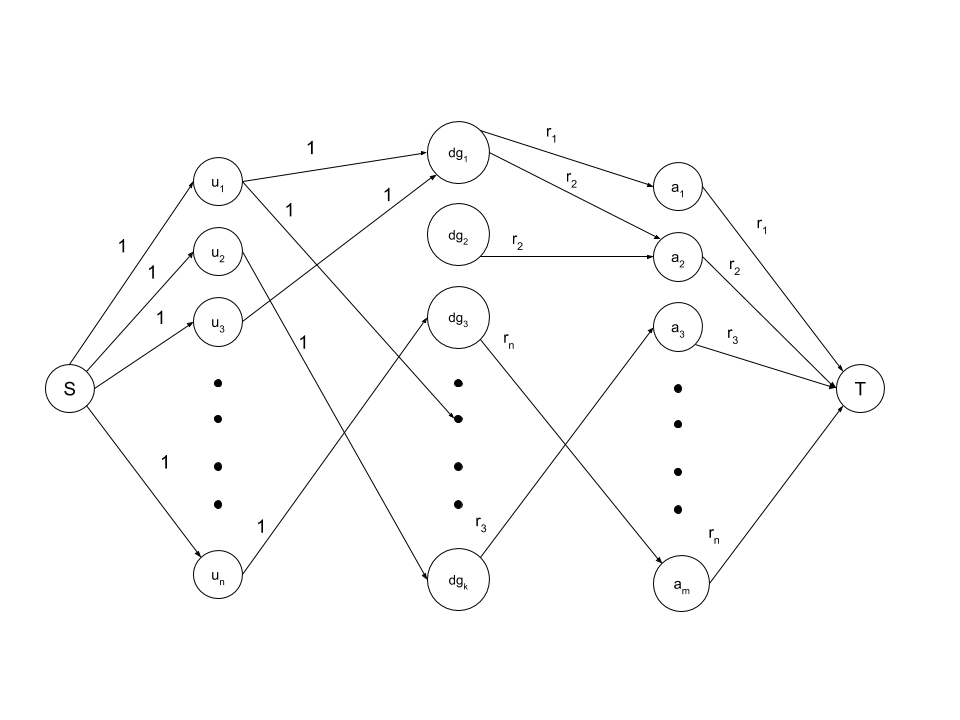
\includegraphics[scale=0.5]{p1hw6}
\subsubsection{
	Algorithm and complexity
}
\begin{algorithm}
	\caption{Satisfy advertisers}
	\Comment{$DG$ is a set containing demographic groups, where each group is denoted as $dg_i$.}
	\Comment{$X$ is a set containing the set of demographic groups that each advertiser wants to target,
		denoted as $X_i$.}
	\Comment{$U$ is a set containing the set of user's demographic groups, denoted as $U_i$}
	\Comment{$r$ is a set containing the minimum number of ads that an advertisers wants to show to a user
		per minute, denoted as $r_i$}
	\Comment{$m$ is the number of advertisers.}
	\Comment{$n$ is the number of users.}
	\Function{ConstructGraph($DG$, $X$, $U$, $r$, $m$, $n$)}{
		Let $V$ be a set of vertices, $E$ be a set of edges\;
		Add $s$ and $t$ to $V$\;
		\Comment{Add users}
		\For{$u_j$ in $U$}{
			Add $u_j$ to $V$\;
			Add edge $(s, u_j)$ to $E$ of capacity $1$\;
		}
		\Comment{Add demographic group}
		\For{$dg_i$ in $DG$}{
			Add $dg_i$ to $V$\;
		}
		\For{$u_j$ in $U$}{
			\For{$dg$ in $U_j$}{
				Add edge $(u_j, dg)$ to $E$ of capacity $1$\;
			}
		}
		\Comment{Add advertisers}
		\For{$i$ from $1$ to $m$}{
			Add $a_i$ to $V$\;
			\For{$dg$ in $X_i$}{
				Add edge $(dg, a_i)$ to $E$ of capacity $r_{i}$\;
			}
			Add edge $(a_i, t)$ to $E$ from of capacity $r_{i}$\;
		}
		\Return{$G=(V,E)$}
	}
	\Comment{The main function}
	\Function{isSatisfied($DG$, $X$, $U$, $r$, $m$, $n$)}{
		$G \leftarrow \FuncCall{ConstructGraph}{$DG$, $X$, $U$, $r$, $m$, $n$}$\;
		Run the Ford Fulkerson algorithm on the network flow graph $G$\;
		\Comment{Check if advertisers can be satisfied, assign user an ad}
		\If{$G$ has a max flow of $\sum_{i=1}^m r_i$}{
			\For{$u_i$ in $G$ where $f^{in}(u_i)=1$}{
				\Comment{user $u_i$, from demographic $dg_k$ will be served an ad from $a_j$ }
				print a path from $u_i \rightarrow dg_k \rightarrow a_j$ that has flow $1$\;
				decrease $f^{in}(a_j)$ by one
			}
			\Return{True}
		}
		\Return{False}
	}
\end{algorithm}
\pagebreak

We claim the time complexity to be $O(|DG|(n+m)+ 
(n + \sum_{i=1}^n|U_i| + \sum_{j=1}^k|DG_j| + m)\sum_{i=1}^m r_i + km|U|)$ for \FuncCall{isSatisfied}{}.
\begin{proof}
\FuncCall{ConstructGraph}{} takes $O(n + |DG| + n|DG| + m|DG|) = O(|DG|(n+m))$ time.
The first for loop takes $n$ time and the second for loop takes $|DG|$ time. 
The third for loop takes $n|DG|$ time because there are $n$ users and the the max amount of elements in $U_j$ is $|DG|$
Similarly, the fourth for loop takes $m|DG|$ time. The rest of the computations take constant time. 

We know in the general case
the Ford Fulkerson algorithm takes, $O(Ef)$ where $E$ is the number of edges and $f$ is the max flow. 
The max number of edges in this graph is $n + \sum_{i=1}^n|U_i| + \sum_{j=1}^k|DG_j| + m$. The max flow is $\sum_{i=1}^m r_i$.
Hence this leads to a time complexity of $O((n + \sum_{i=1}^n|U_i| + \sum_{j=1}^k|DG_j| + m)\sum_{i=1}^m r_i)$

Checking the if statement takes $2m$ time because computing that max flow takes $m$ time and checking if 
$G$ has such max flow takes checking all the incoming edges into $T$ which takes $m$ time.  
The for loops runs $|U|$ times and in each loop we print a path. Search for such a path using breath first search 
takes $km$ time. The rest of the computations take constant time. Thus the total for loop takes $km|U|$ time
and the time complexity of the this algorithm following the Ford Fulkerson takes $O(2m + km|U|) = O(km|U|)$.


Taking all these values together, the total time complexity is $$O\Bigg(|DG|(n+m)+ 
(n + \sum_{i=1}^n|U_i| + \sum_{j=1}^k|DG_j| + m)\sum_{i=1}^m r_i + km|U| \Bigg)$$.

\end{proof}


\subsection{
	Present the analysis on the correctness of your algorithm.
}

\subsubsection{
	Show that a solution to the original problem will result in flows (i.e. satisfies
	the conservation and capacity conditions) in the network flow graph $G$.
}
\begin{proof}
	Suppose there exists an assignment of ads to users such that all advertisers are satisfied.
	%Consider the solution where each advertiser $a_i$, will have $r_i$ ads shown to one
	%demographic group, $dg_k \in X_i$.
	We will show that we can obtain an $s-t$ flow from such assignment.

	Let there be $r_i$ number of user nodes, $u_j$, that belong to demographic group $dg_\lambda$ for each
	advertiser $a_i$. For each $u_j$ and its advertiser $a_i$, consider the flow that sends one unit
	along each path of $s \rightarrow u_j \rightarrow dg_\lambda \rightarrow a_i \rightarrow t$.
	Let $f(e)=1$ for each $s \rightarrow u_j$ and $u_j \rightarrow dg_\lambda$ edge.
	By definition, conservation condition holds for all $u_j$.
	The capacity condition holds for all $s \rightarrow u_j$ and $u_j \rightarrow dg_\lambda$ edges
	because the capacities of those edges is $1$.

	%We know that $f^{in}(a_i) = r_i$ because all advertisers are satisfied.
	We know that $f^{in}(dg_\lambda)$ will be equal to total number of users such that 
	all advertisers will be satisfied, i.e. the number of ads from $dg_\lambda$ that $a_1$ wants 
	plus the number of ads from $dg_\lambda$ that $a_2$ wants, $\cdots$, 
	plus the number of ads from $dg_\lambda$ that $a_m$ wants. 
	Let $f(e)=\zeta$ for each $dg_\lambda \rightarrow a_i$, where $\zeta$ is the number of ads 
	that $a_i$ wants from demographic group $dg_\lambda$.
	Hence, conservation condition holds for all $dg_\lambda$.
	The capacity condition holds for all $dg_\lambda \rightarrow a_i$ because
	because the capacities of those edges is equal or less $r_i$ because the total number of
	ads from $dg_\lambda$ that $a_i$ wants is equal or less than $r_i$.

	Let $f(e)=r_i$ for each $a_i \rightarrow t$. Hence, conservation condition holds for all $a_i$.
	The capacity condition holds for all $a_i \rightarrow t$ because
	because the capacities of those edges is $r_i$.

	Therefore, there exists an assignment of ads to users such that all advertisers are satisfied
	which results in a flow network. If all advertisers are satisfied, the total $s \rightarrow t$ flow
	will be $\sum_{i=1}^m r_i$. Otherwise, it will be less than the previous sum with flows less than $r_i$
	on edges $a_i \rightarrow t$.
\end{proof}


\subsubsection{
	Show that the solution to the network flow problem will give the solution for
	the original problem.
}


\begin{proof}
	Suppose we have a solution with the $s \rightarrow t$ flow being $\sum_{i=1}^m r_i$.
	This means that $f(e) = r_i$ for at all edges $a_i \rightarrow t$ as the this is the only
	way to get total flow of $\sum_{i=1}^m r_i$. Consequently, this means we have identified
	$r_i$ users for each $a_i$ advertiser.  Thus, all advertisers will be satisfied.

	If the algorithm gives us a maximum $s \rightarrow t$ flow that is less than $\sum_{i=1}^m r_i$,
	it means $f(e) < r_i$ for at least one edge $a_i \rightarrow t$.
	Thus, some advertiser will not have the number of ads shown to users they requested.
	That is why in this case we can claim that there doesn't exist enough users such that
	all advertisers are satisfied.
\end{proof}




\pagebreak
%7.26



\section{
  Give a polynomial-time algorithm to decide whether it is possible to
  keep the set of phones fully connected at all times during the travel of
  this one cell phone.
 }

\subsection{
	Construct a network flow model for this problem. Clearly state the
	meaning of each component (node, edge, capacity) of the flow network that you
	construct, present your algorithm in pseudocode, and give the computing complexity
	analysis of your algorithm.
}
We construct a bipartite graph $BP=(P \cup B,E)$ to model the network flow.
\subsubsection{
	Components for graph
}
\begin{enumerate}[label=\alph*.]
	\item{
	      \textbf{Nodes}
	      \begin{itemize}
		      \item Add a column of $n$ nodes, denoted as $p$, to represent the number of cellular phones. The set of all phones will be denoted as $P$.
		      \item Add a column of $k$ nodes, denoted as $b$, to represent the number of base stations. The set of all base stations will be denoted as $B$.
	      \end{itemize}
	      }
	\item{
	      \textbf{Edges and capacities}
	      \begin{itemize}
		      \item{
		            Add edges $p_i \rightarrow b_j$ if the distance from $p_i$ to $b_j$ is at most $\Delta$.
		            Set the capacity of these edges to be $1$.
		            }
	      \end{itemize}
	      }
\end{enumerate}
The corresponding flow network $G$, will have a node $s$, with outgoing edges to all $p$ of capacity $1$, and
have a node $t$, with incoming edges from all $b$ of capacity $1$.
\begin{center}
	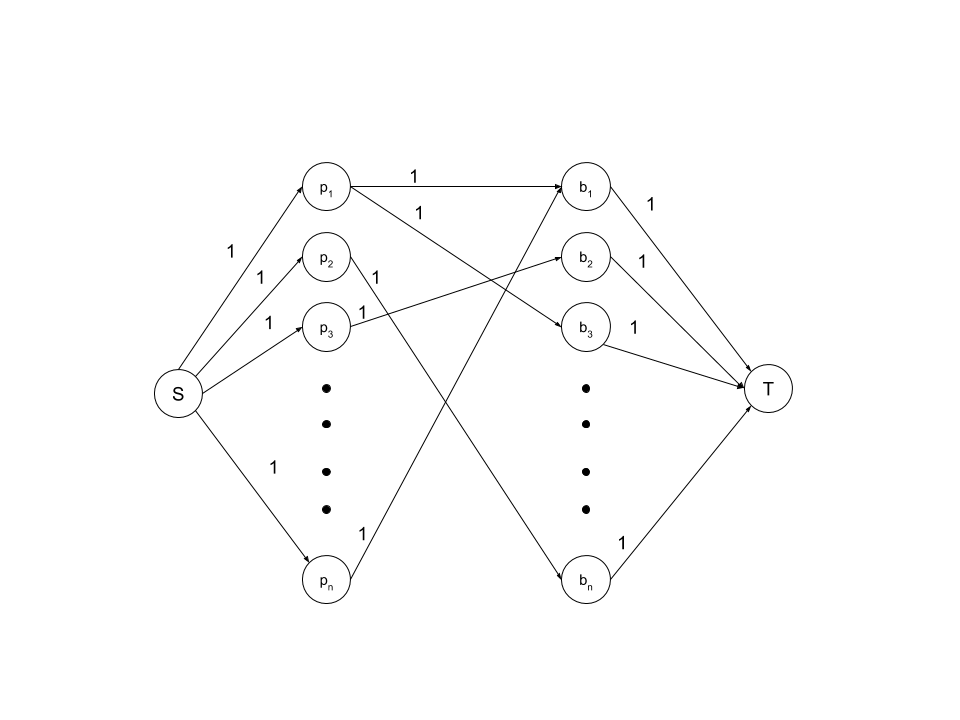
\includegraphics[scale=0.4]{p2hw6}
\end{center}

\subsubsection{
	Naive algorithm
}

We can model the movement of phone $p_1$ by constructing a new graph it moves one unit east.
Let $G_0$ model the state of the cellular network before any movement occurs in phone $p_1$.
$G_1$ will represent the state of the cellular network where phone $p_1$ has moved one unit east.
We update edges of $p_1$ such that the distance from $p_1$ to $b_j$ is at most $\Delta$ given the
new location. We will have a total of $z$ graphs. If all graphs have perfect matching, there exists
an assignment such that all phones will be connected during the movement of $p_1$.

According Theorem 7.40, we know that we can compute if a perfect match exists in $O(mn)$ time, where $m$ is the
number of edges and $n$ is the number of nodes. We know that $m \leq n^2$ because $n^2$ is the maximum
amount of edges we can have in this bipartite graph. Hence, computing if a perfect match exists for one graph
takes $O(n^3)$ time. Since we have $z$ graphs, the total time to compute this algorithm will take $O(zn^3)$ time.

\subsubsection{
	Faster algorithm
}

Suppose there exists a perfect match on graph $G_\phi$.
Notice that we can reuse the matchings we have previously computed for $G_{\phi}$ to compute
matchings for $G_{\phi+1}$. If we update the edges of $p_1$ to state $\phi +1$ in graph $G_{\phi}$,
the amount of matches either stays at $n$ or decreases to $n-1$. If the amount of matches stays at $n$,
a perfect match exists at state $\phi + 1$ and we are done. If the amount of matches are $n-1$, we
compute a augmenting path to see if we can increase the matches to $n$. Computing a single
augmenting path takes $O(m) = O(n^2)$.

Hence our total time complexity will be computing matches for $G_0$, which takes $O(n^3)$,
and computing augmenting paths for the following $z$ state changes, which takes $O(zn^2)$.
This leads to a total time complexity of $O(n^3 + zn^2) = O(n^3)$, as desired.


\iffalse
	If it is possible, you should report a sequence
	of assignments of phones to base stations that will be sufficient in order
	to maintain full connectivity;
\fi
\begin{algorithm}
	\caption{Full connectivity}
	\Comment{$P$ is a set containing the location of each phone, denoted as $P[i]$}
	\Comment{$B$ is a set containing the location of each base station, denoted as $P[i]$}
	\Comment{$\Delta$ is the range parameter}
	\Function{ConstructGraph($P, B, \Delta$)}{
		Let $V$ be a set of vertices, $E$ be a set of edges\;
		Add $s$ and $t$ to $V$\;
		\Comment{Add phones}
		\For{$i$ from $1$ to $|P|$}{
			Add $u_i$ to $V$\;
			Add edge $(s, u_i)$ to $E$ with capacity $1$\;
		}
		\Comment{Add base stations}
		\For{$j$ from $1$ to $|B|$}{
			Add $b_j$ to $V$\;
			Add edge $(b_j, t)$ to $E$ with capacity $1$\;
		}
		\Comment{Add edges}
		\For{$i$ from $1$ to $|P|$}{
			\For{$j$ from $1$ to $|B|$}{
				\If{distance from $P[i]$ to $B[j]$ is at most $\Delta$}{
					Add edge $(p_i, b_j)$ to $E$ with capacity $1$\;
				}
			}
		}

		\Return{$G=(V,E)$}
	}
	\Comment{The main function}
	\Comment{$z$ is units of distance that phone $p_1$ travels east}
	\Function{fullConnectivity($P, B, z, \Delta$)}{
		$S \leftarrow$ a list to store sequences
		of assignments of phones to base stations that will be sufficient in order
		to maintain full connectivity\;
		$G \leftarrow \FuncCall{ConstructGraph}{$P, B, \Delta$}$\;
		Run the Ford Fulkerson algorithm on the network flow graph $G$\;
		\If{$G$ has a max flow of $|P|$}{
			$S[0] \leftarrow$ add the current perfect matching
		}
		\Else{
			print no possible matches for the initial state
		}
		\For{$i$ from $1$ to $z$}{
			$G \leftarrow$ update $p_1$'s edges so that it reflects its new position (1 unit east)\;
			\If{$G$ has a max flow of $|P|$}{
				$S[z] \leftarrow$ add the current perfect matching
			}
			\Else{
				$G \leftarrow$  Run one iteration of Ford Fulkerson to compute an augmenting path\;
				\If{$G$ has a max flow of $|P|$}{
					$S[z] \leftarrow$ add the current perfect matching
				}
				\Else{
					print no possible matches for the $z$th state
				}
			}
		}
		\Return{$S$}
	}
\end{algorithm}

\pagebreak

Time complexity yadada
$2n + n^2$ for generating graph

\subsection{
	Present the analysis on the correctness of your algorithm.
}

\subsubsection{
	Show that a solution to the original problem will result in flows (i.e. satisfies
	the conservation and capacity conditions) in the network flow graph $G$.
}
\begin{proof}
	Suppose there exists an assignment of edges such that all phones will be connected to a base station.
	We will show that we can obtain an $s-t$ flow from such assignment.

	For each phone $p_i$ and the base station $b_j$ it's connected to, consider the flow that sends one unit
	along each path of $s \rightarrow p_i \rightarrow b_j \rightarrow t$. Let $f(e)=1$ for all edges.
	The capacity condition holds for all edges because we defined the capacities to be $1$.
	The conservation condition holds for $p_i$ and $b_j$ because the flow entering and leaving the nodes is both $1$.

	Therefore, there exists an assignment of edges such that all phones will be connected to a base station
	which results in a flow network. If all phone are connected, the total $s \rightarrow t$ flow
	will be $n$. Otherwise, it will be less than the $n$ with empty flows on edges $b_j \rightarrow t$.
\end{proof}


\subsubsection{
	Show that the solution to the network flow problem will give the solution for
	the original problem.
}


\begin{proof}
	Suppose we have a solution with the $s \rightarrow t$ flow being $n$.
	This means that $f(e) = 1$ for at all edges $p_i \rightarrow b_j$ as the this is the only
	way to get total flow of $n$. Consequently, this means we have identified
	a base station for all phones.  Thus, all phone can be connected.

	If the algorithm gives us a maximum $s \rightarrow t$ flow that is less than $n$,
	it means $f(e) < 1$ for at least one edge $p_i \rightarrow b_j$.
	Thus, some phones cannot connect to a base station.
	That is why in this case we can claim that there doesn't exist stations such that
	all phones can be connected.
\end{proof}




\end{document}

